\par
We will discuss about out our dataset, how we acquired it and what we made it feasible for the analysis, means data preprocessing. Data acquisition and data preprocessing are very important steps because the performance of any ML model depends largely on data quantity and data quality. Acquiring, cleansing, and organizing data are so important steps that scientists usually put around 80\% of their efforts in these data related tasks. This is because of the fact that in the real world data set is collected from various sources such as a files, websites, database, sensors and much more. Also, the collected data can be inconsistent, incomplete and/or noisy. This can happen for many several reasons. First of all there can be data entry problems like people just essentially type things incorrectly. There could be data transmission problems like when the data is sent between different databases or companies, things can get lost in the process. Also, there could be data collection problems like someone simply might not have collected some of the data or have collected incorrectly. Therefore, we need to modify and clean the acquired unformatted real-world data. This can be done through ignoring the missing record, filling the missing values manually, filling using computed values, data binning, smoothing of data using a specified linear function, detected outliers by grouping, removing noisy data manually, etc. Then this pre-processed data can be used to train a ML model.
\newline
\par
In our case, instead of acquiring data from internet or any other sources, we are simulating our data by writing a program. This gives us more control over the quantity and quality of data. In this chapter, we will discuss in detail how we generated our data, what are advantages and limitations of this approach, and how we prepared it for our predictive ML model.

\section{Data Gathering}
\par
Since our thesis goal was to analyze traffic scene, we obviously needed a large amount of traffic data. There has been a huge boost in traffic lane related research in the past two decades but many of the datasets are private. High-quality labeled data in abundance is always costly in both time and money to acquire. For the cases where we just cannot get enough labeled data we simulate data. Therefore, we have developed a Traffic Simulator using a gaming engine called Unity3D \ref{subsec:unity}, for AI research to experiment with computer vision and deep learning for autonomous vehicles. It captures screenshots of our simulation after each time interval and saves it. We can increase and decrease the time intervals as well. There are lot of advantages of developing this simulation compared to real-world data. We have a total control on our data. We can re-enact any scenario, that happens in the real-world, in our simulation. We can simulate anything in a traffic scene that helps in autonomous vehicle research like the weather conditions, lighting conditions, road length, types of obstacles and types of vehicles. The possibilities are endless. But we have to modify the program to incorporate these changes. However, our system exposes a simple configuration file, as shown here \ref{lst:config_file}, through which we can modify certain aspects of the simulation very easily. For example, number of lanes, road type (curve or straight), length of road, sharpness of turn, elevation of road, speed of ego vehicle, maximum and minimum number of vehicles on road.
\par
\begin{listing}i
  \inputminted[frame=lines,framesep=2mm,baselinestretch=1.2,fontsize=\scriptsize,linenos]{json}{Chapter3/config.json}
  \caption{Data generation Configuration file}
  \label{lst:config_file}
\end{listing}
\par
We are using supervised learning approach to solve our problem. As we explained earlier, for supervised learning, we need labelled training data. So first of all we need to generate our Dataset and the respective Labels. Then we can do prepare our data for our choosen model.

\subsection{Dataset}
We have developed a simple Traffic Simulator using Unity3D \ref{subsec:unity} to simulate traffic scenes and capture data through it. The simulation heavily uses the EasyRoad3d \ref{subsec:easyroad3d} toolset for the creation of road network, vehicles, side objects and terrain. The road type we set up is undivided or bi-directional with a minimum of 1 lane and a maximum of 4 lanes. The side objects included in our simulation are houses and trees. We have written custom scripts to modify the behaviour of the simulation such as: to take screenshots at regural interval of time, handling configurtion files \ref{lst:config_file} and generating the environment accordingly.
\par
In order to run our simulation, we just need to click Play button as shown in our Unity3d environment in Figure \ref{unity_environment}. Then, just like in racing games, we can use arrow keys to control movement of our ego vehicle (the vehicle we are controlling).
\par
\begin{figure}[H]
  \centering
  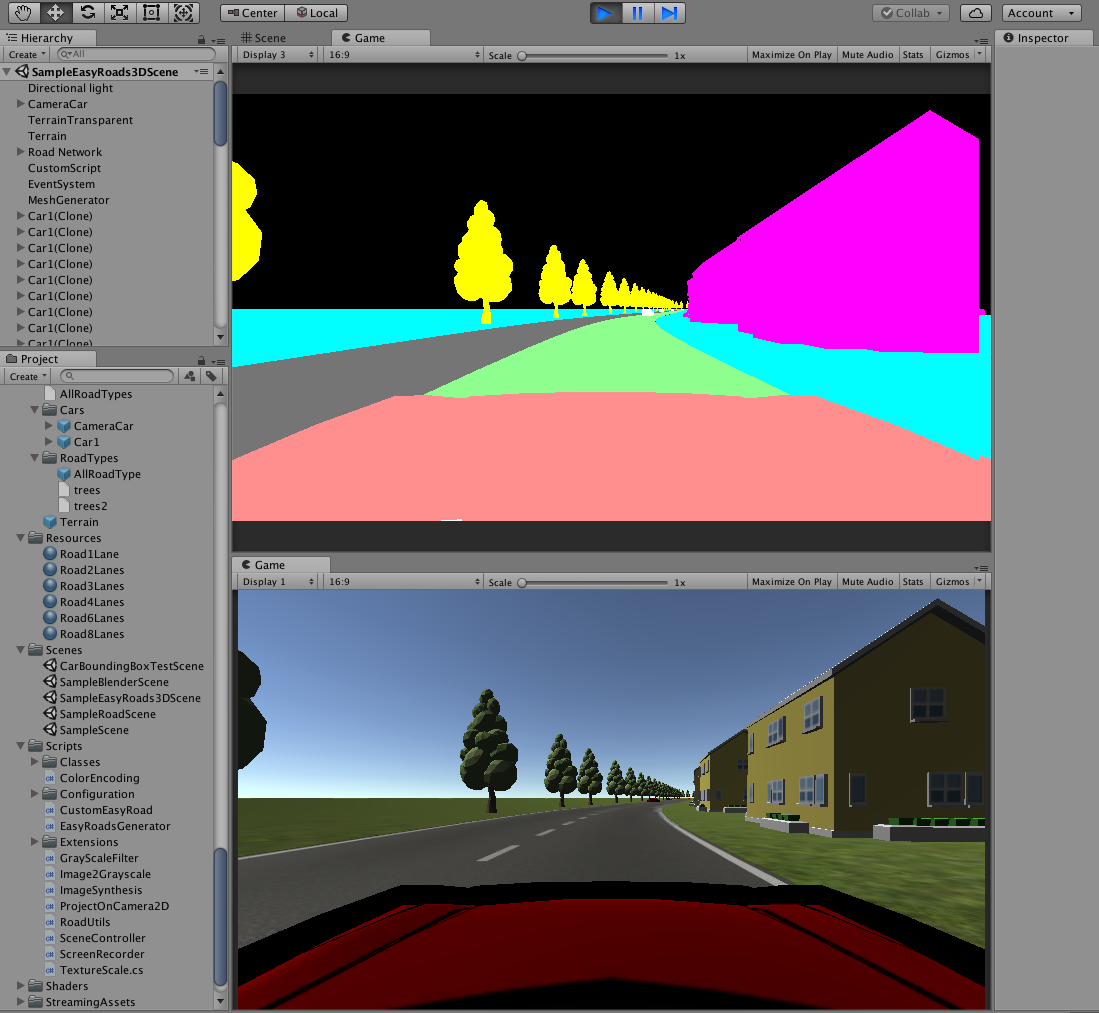
\includegraphics[scale=0.40]{images/Chapter3/unity_environment.png}
  \caption{Unity3D Environment}
  \label{unity_environment}
\end{figure}
\par
The simulator takes screenshots of the traffic scene after regular time intervals of time and save into a directory. Also, the scenes captured are from the viewing point of a dashboard camera and ego-vehicle being in the rightmost lane. Although, we have kept our simulation simple because our focus of study is only lane detection, we could have made a traffic scene more complex by following things by adding:
\begin{itemize}
  \item Pedestrians and bicyclists
  \item Different vehicles
  \item Traffic signs and signals
  \item Different lighting conditions
  \item Side objects like different kinds of trees, fire hydrants, foot paths, etc.
  \item Changing Weather conditions
  \item Crosswalks, roundabouts and road intersections
\end{itemize}

\par
We ran our simulator multiple times with different configurations for example, with different number of lanes. The images of traffic scene we captured can be categorized into the following table:
\begin{table}[H]
\centering
\begin{tabular}{l | l }
No. of Lanes & No. of Images\\
\hline
Lane 1 & 4000 \\
Lane 2 & 4000 \\
Lane 3 & 4000 \\
Lane 4 & 4000 \\
\hline
Total Images & 16000
\end{tabular}
\caption{Overview of number of images generated for 1-4 lanes of simulated traffic scene}
\label{dataset_count}
\end{table}
All the images gathered are of size 1280x720 pixels and JPEG format and are stored in separate directories according to the maximum number of lanes. Sample images from each category, respective to maximum number of lanes in a scene, are shown below:
\begin{figure}[H]
  \centering
	\begin{subfigure}[b]{0.6\linewidth}
		\centering
    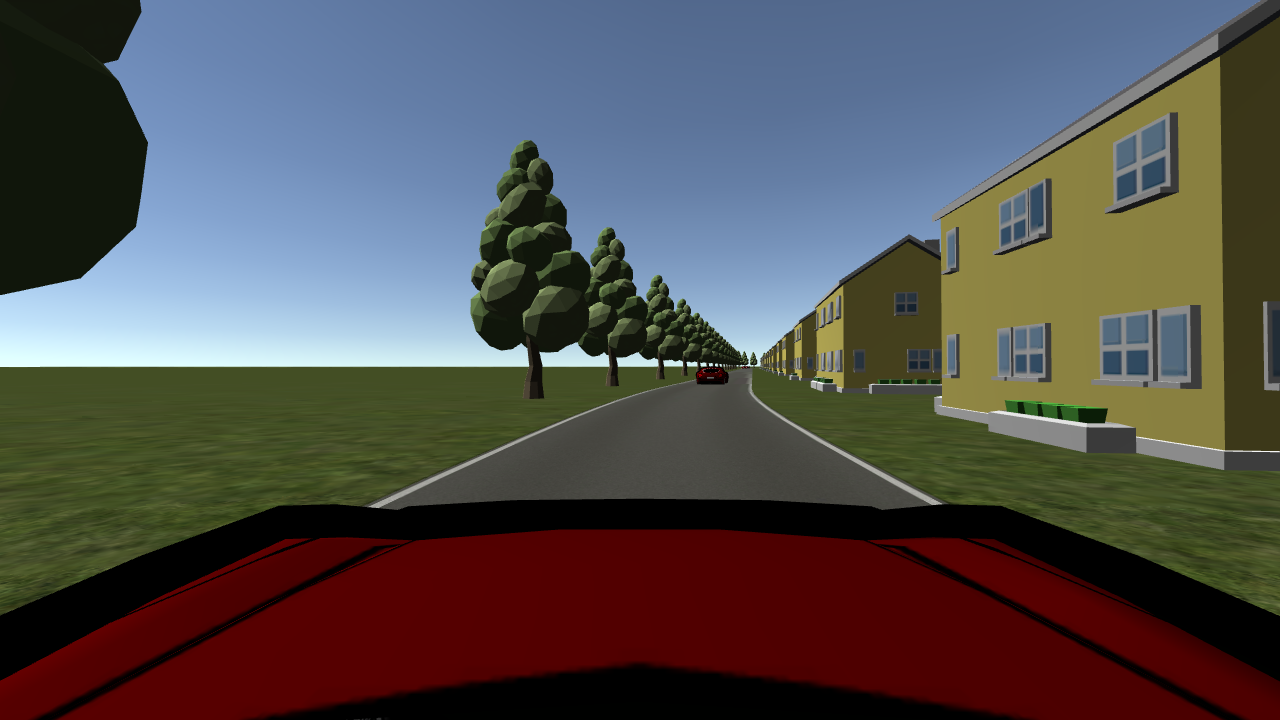
\includegraphics[width=\textwidth]{images/Chapter3/lane1.jpg}
    \caption{Max. Lane = 1}
	\end{subfigure}\hfill
  
  \begin{subfigure}[b]{0.6\linewidth}
		\centering
    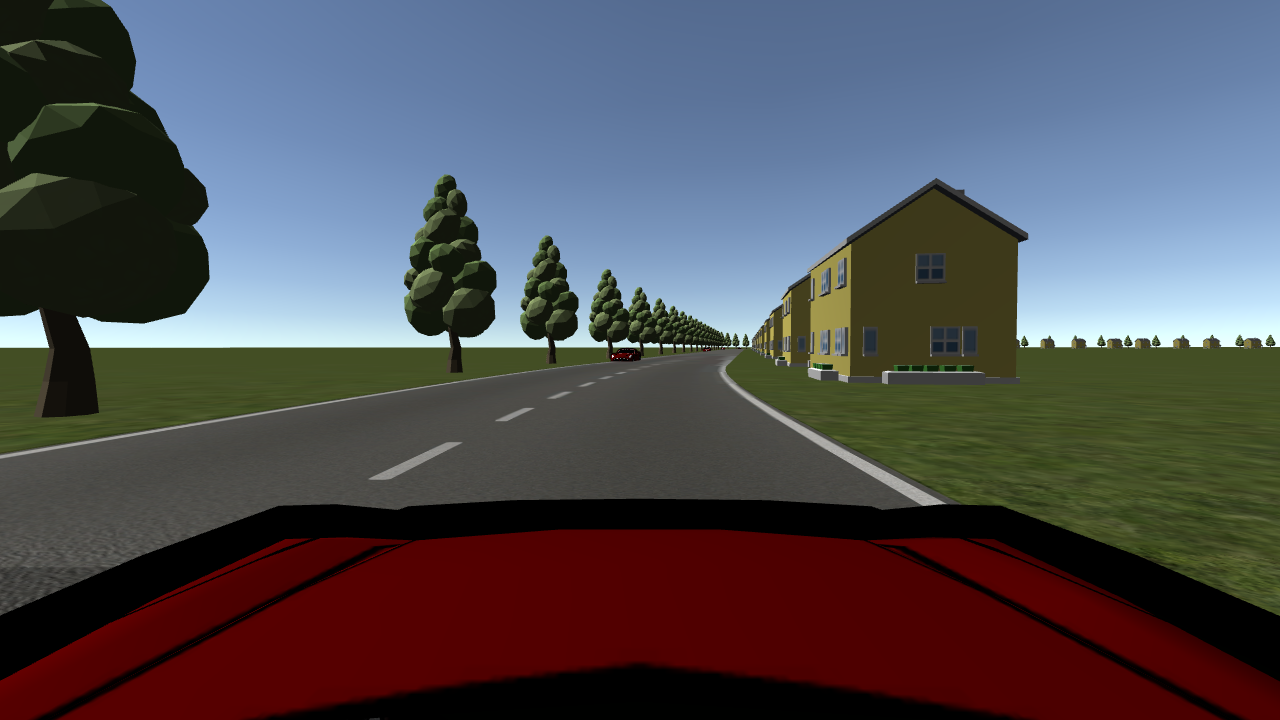
\includegraphics[width=\textwidth]{images/Chapter3/lane2.jpg}
    \caption{Max. Lane = 2}
	\end{subfigure}\hfill
  
  \begin{subfigure}[b]{0.6\linewidth}
		\centering
    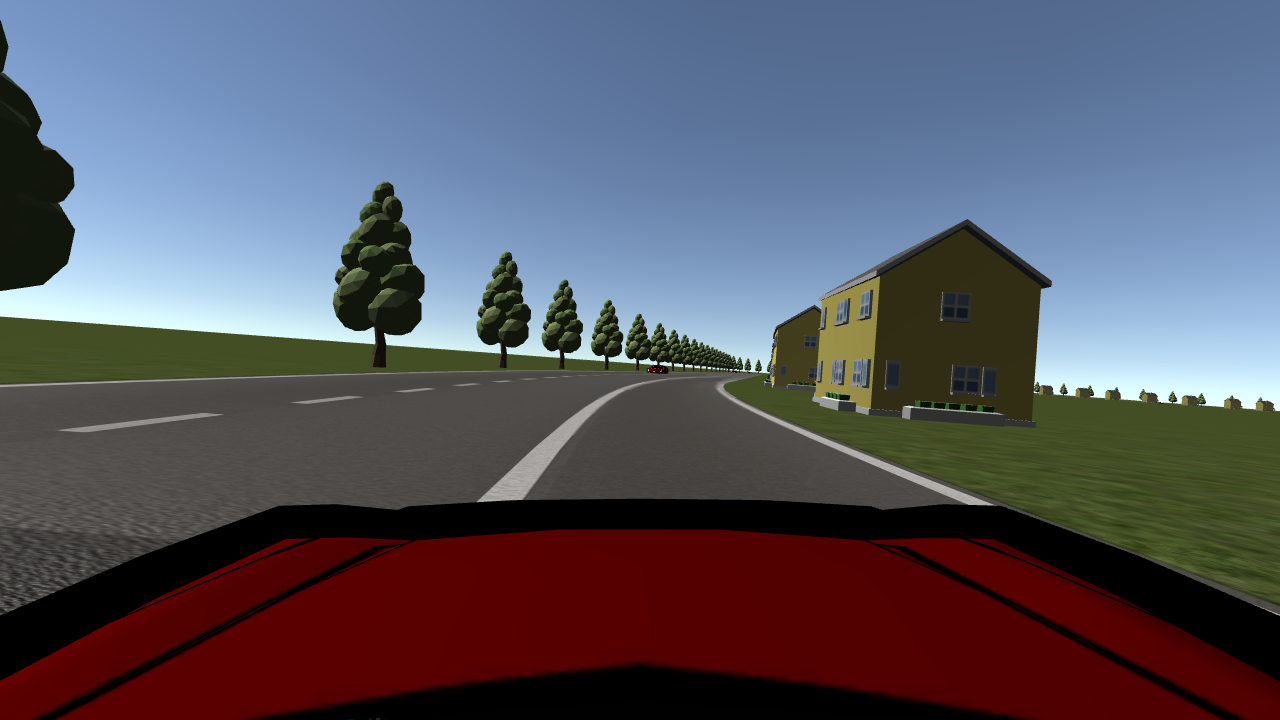
\includegraphics[width=\textwidth]{images/Chapter3/lane3.jpg}
    \caption{Max. Lane = 3}
	\end{subfigure}\hfill
 
	\begin{subfigure}[b]{0.6\linewidth}
		\centering
    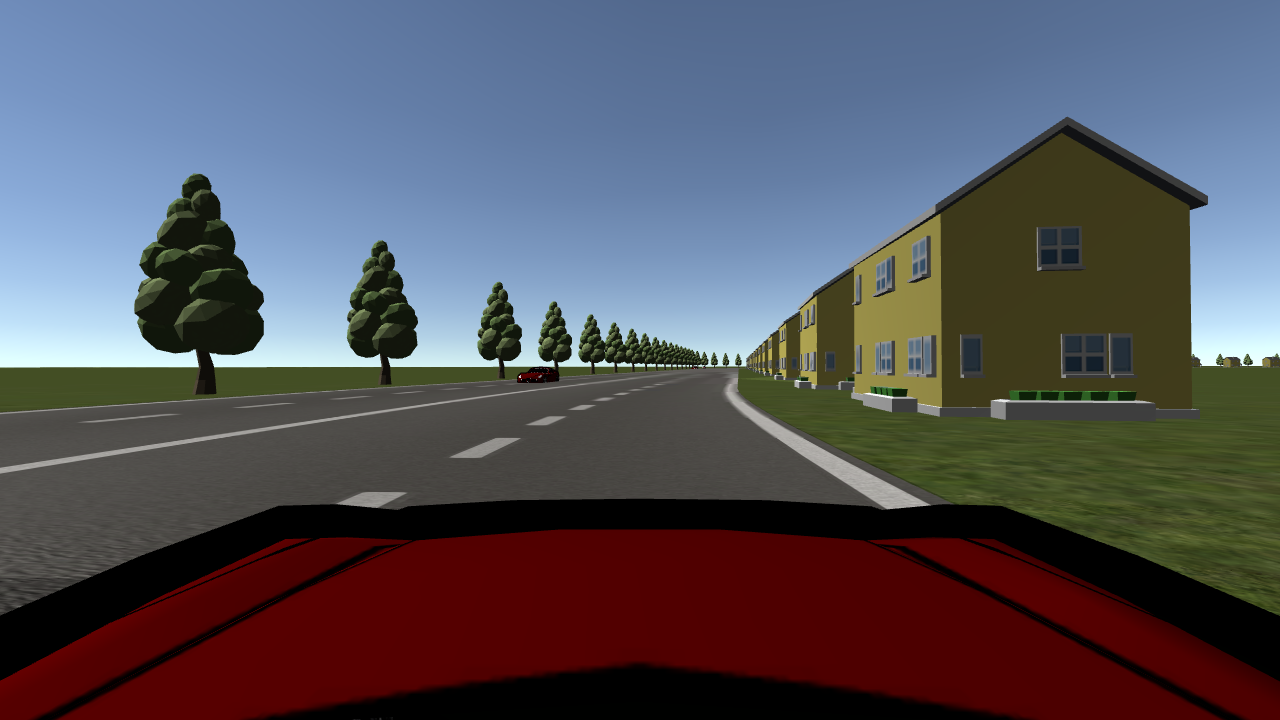
\includegraphics[width=\textwidth]{images/Chapter3/lane4.jpg}
    \caption{Max. Lane = 4}
	\end{subfigure}
	\caption{Gathered images of Traffic scenes}
  \label{}
\end{figure}

\subsection{Labels}
Since we are gathering all the images in separate directories according to the maximum number of lanes present in the image, we can easily get the labels from the folder name. For example, if we use the configuration file as shown here \ref{lst:config_file}, then run the simulator we developed, it will capture all the screenshots in a folder. We can say that all the image files in that folder have 3-lanes road because the configuration file has \q{NumberOfTracks} set to 3. Then, using a small Python script we can append \q{-3} to every file in that folder. In similar fashion, we can set \q{NumberOfTracks} to a different value from 1 to 4, generate images and append labels to each image file. Hence, each image file will have its label at the end of its name. These image wise labels are needed to predict maximum number of lanes present in an image.

However, our focus is to predict to which lane a specific pixel of an image belongs to. For that we need pixel wise labels. Since the engine is generating these scenes, it can simultaneously generate the suitable labels, such as segmentation masks or bounding boxes. Unity offers an open-source package known as \q{Image Synthesis for Machine Learning} \cite{unity_image_synthesis}. The goal of this project is to help researchers in machine learning and computer vision produce annotated training sets in Unity. It is the perfect starting point for the development of synthetic image generators. This project's repository includes code that can be easily incorporated into any existing Unity project. It makes it possible to store image segmentation, optical flow, depth, etc. as RGB encoded image file in PNG format with negligible interference in the current simulation:
\begin{itemize}
  \item \textbf{Image segmentation} - each object in the scene gets unique color
  \item \textbf{Depth} - pixels are colored according to their distance from the camera
  \item \textbf{Normals} - surfaces are colored according to their orientation in relation with the camera
  \item \textbf{Optical flow} - pixels are colored according to their motion in the relation to camera
  \item \textbf{Object categorization} - objects are assigned color based on their category
\end{itemize}
We were able to incororate the Image Synthesis project by following the steps mentioned the project's description \cite{unity_image_synthesis_description}. A sample snapshot of a simulated driving scenario, as shown in the Figures \ref{fig:lane_4}, and the various annotations or labels, as shown in the Figures \ref{fig:image_segmentation} \ref{fig:depth} \ref{fig:normals}, are collected automatically. Every frame and multiple annotations per frame can be stored on a disk by the provided scripts. The project does not include the car simulator, the figures shown below are captured from our simulation. All the images captured are of size 1280x720 pixels. We are only using the original image as training data and segmented image to get pixel-wise labels, to train our neural network. However, other annotation images: Depth, Normals and Optical flow can be used for further research.

\begin{figure}[H]
  \centering
  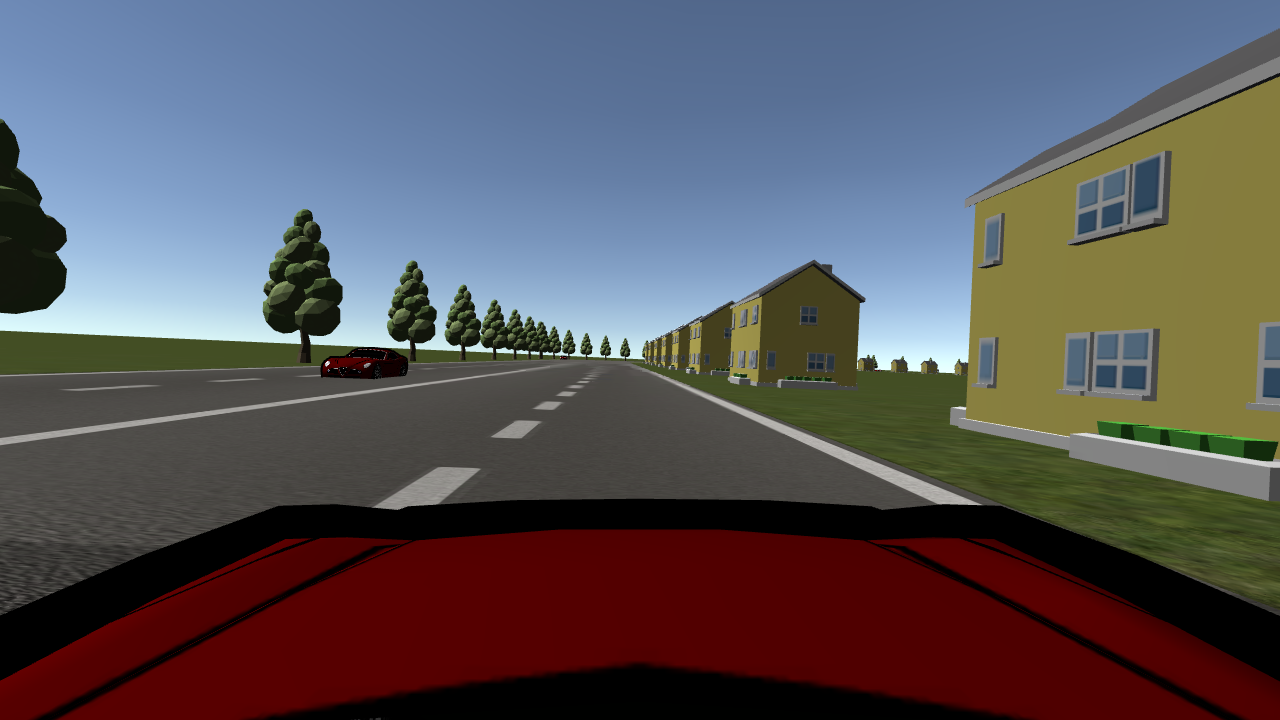
\includegraphics[width=\textwidth]{images/Chapter3/_img.jpg}
  \caption{4-Lane Roadway}
  \label{fig:lane_4}
\end{figure}
\begin{figure}[H]
  \centering
  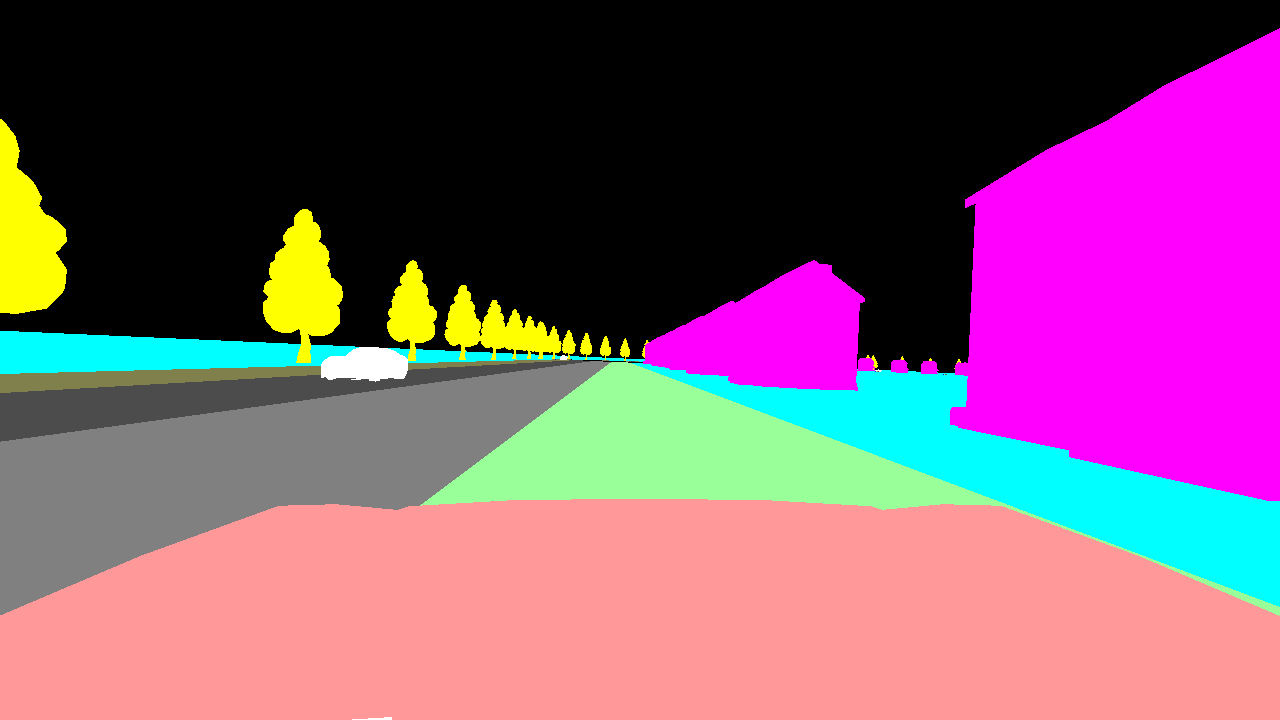
\includegraphics[width=\textwidth]{images/Chapter3/_layer.jpg}
  \caption{Image segmentation}
  \label{fig:image_segmentation}
\end{figure}
\begin{figure}[H]
  \centering
  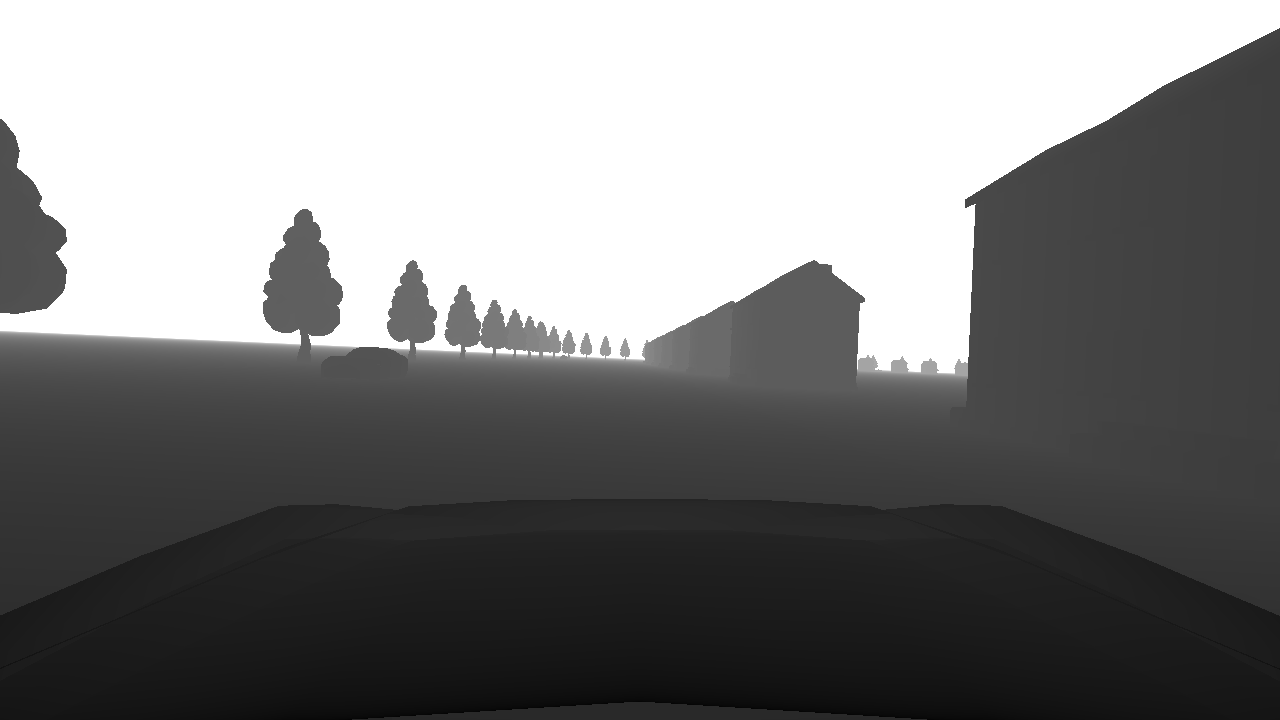
\includegraphics[width=\textwidth]{images/Chapter3/_depth.jpg}
  \caption{Depth}
  \label{fig:depth}
\end{figure}
\begin{figure}[H]
  \centering
  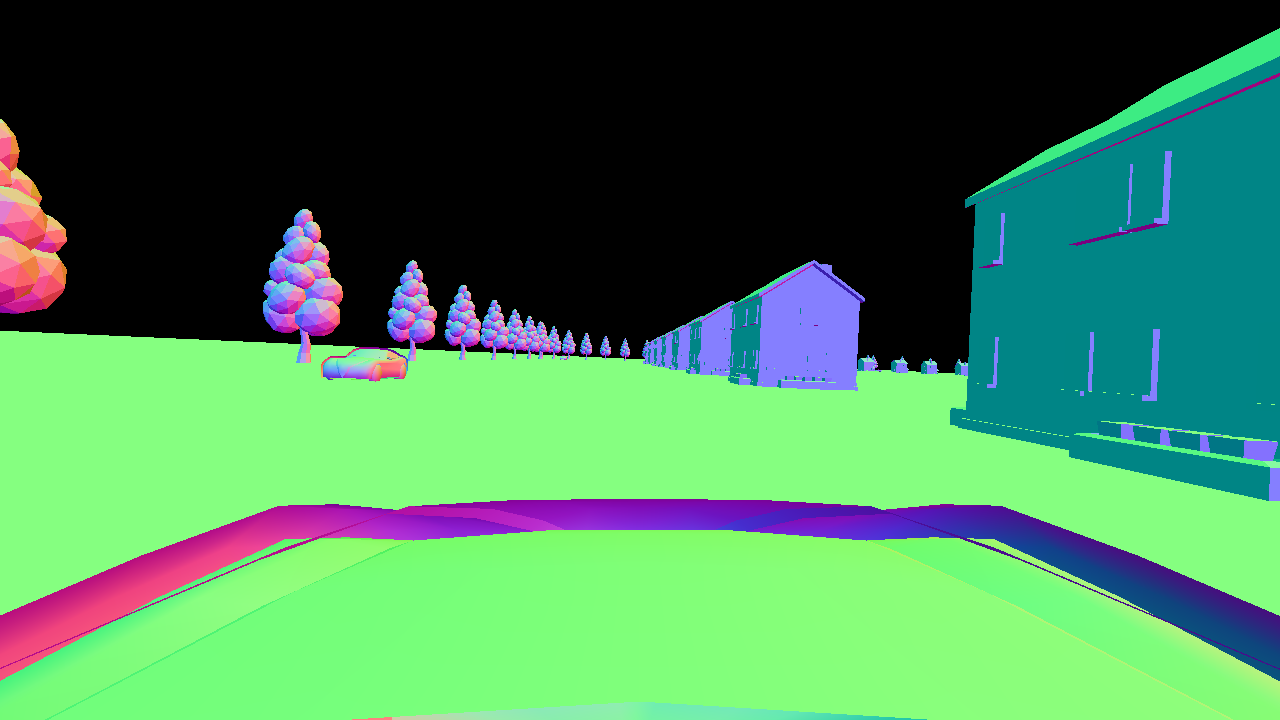
\includegraphics[width=\textwidth]{images/Chapter3/_normals.jpg}
  \caption{Normals}
  \label{fig:normals}
\end{figure}
\begin{figure}[H]
  \centering
  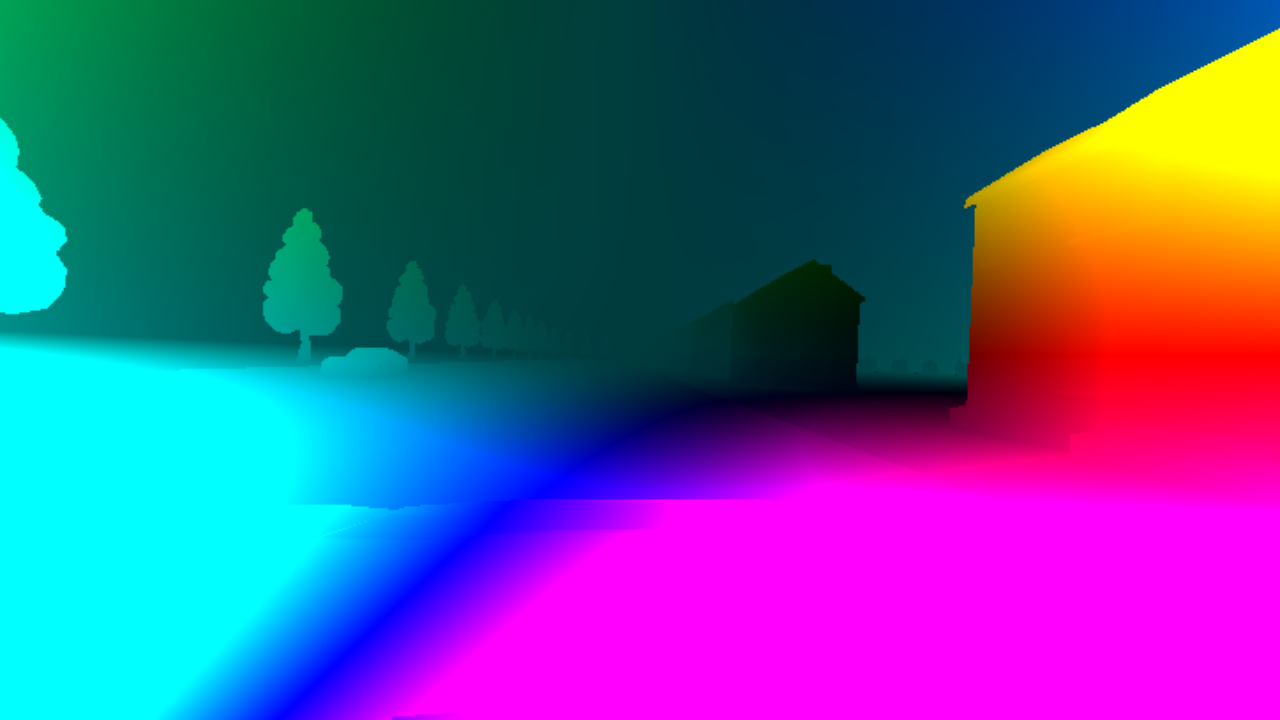
\includegraphics[width=\textwidth]{images/Chapter3/_flow.jpg}
  \caption{Optical flow}
  \label{fig:flow}
\end{figure}

\section{Data Pre-processing}
% minify-images -> image-to-numpy -> generate-random-points -> hot-vector -> learn-point

Data preprocessing is a process that involves transforming raw data into an understandable format for the machine learning algorithm. It is a vital step in the machine learning pipeline \ref{ml-pipeline} and leads to better models and predictions.

Models with small-images are much faster to train. After all an image input size twice as large has four times as many pixels to learn on. The images we captured in Data Gathering process are of 1280x720 pixels in size. So for our initial input size we will choose 1/5 of that: 256x144. If our classifier that does not performs well on tiny n x n (256 x 144) images, we can also scale our model up to 2n x 2n (512 x 288) images. So in the first step, we resize all the input and segmented images to 256x144 pixels and copied into separate folders \q{images\_train} and \q{images\_segmented}, respectively.

In our simulation we have different kinds of objects namely sky, terrain, trees, houses, other cars, ego-car and the road. Hence, we have separate color for each object in the segmented image. Since we are detecting the lanes in this study, the road is further color segmented into lanes. Following is the list of segments and their color-code in our segmented images:

\begin{table}[H]
  \centering
  \begin{tabular}{ |c|c| }
    \hline
    \textbf{Segment} & \textbf{RGB Color Code} \\
    \hline
    Sky & rgb(   0,   0,   0) \\
    \hline
    Terrrain & rgb(   0, 255, 255) \\
    \hline
    Tree & rgb( 255, 255,   0) \\
    \hline
    House & rgb( 255,   0, 255) \\
    \hline
    Other-cars & rgb( 255, 255, 255) \\
    \hline
    Ego-car & rgb( 255, 153, 153) \\
    \hline
    Lane-1 & rgb( 153, 255, 153) \\
    \hline
    Lane-2 & rgb( 128, 128, 128) \\
    \hline
    Lane-3 & rgb(  76,  76,  76) \\
    \hline
    Lane-4 & rgb( 128, 128,  76) \\
    \hline
  \end{tabular}
\caption{Color segmentation}
\label{color_code}
\end{table}

The lane 1 is right-most lane and lane 4 is left-most lane in our dataset. Then we generated random 1200 pixel coordinates for each image and get pixel-wise label using the segmented image. After that we randomize it store it in a file so it can be used in our model training process.